\documentclass[tikz,border=2pt]{standalone}
\usepackage{amsmath}
\usetikzlibrary{arrows.meta}
\begin{document}
% The four classes of games by timing (static/dynamic) and information (complete/incomplete),
% with the solution concept used for each class and the course weeks (1-2, 3-4, 5-6, 7).
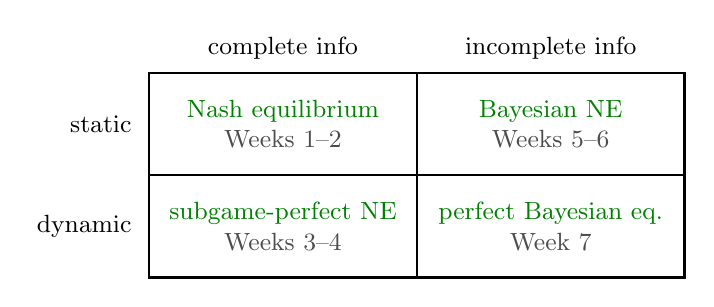
\begin{tikzpicture}[font=\small, >={Latex[length=2mm]},
    cell/.style={align=center, text width=3.1cm}]
  \def\w{3.4} \def\h{1.3}
  \draw[thick] (0,-\h) rectangle (2*\w,\h);
  \draw[thick] (\w,-\h) -- (\w,\h);
  \draw[thick] (0,0) -- (2*\w,0);
  % headers
  \node[anchor=south] at (0.5*\w,\h+0.05) {complete info};
  \node[anchor=south] at (1.5*\w,\h+0.05) {incomplete info};
  \node[anchor=east] at (-0.1,0.5*\h) {static};
  \node[anchor=east] at (-0.1,-0.5*\h) {dynamic};
  % cells: solution concept and course weeks
  \node[cell] at (0.5*\w,0.5*\h) {\textcolor{green!50!black}{Nash equilibrium}\\ \textcolor{gray!60!black}{Weeks 1--2}};
  \node[cell] at (1.5*\w,0.5*\h) {\textcolor{green!50!black}{Bayesian NE}\\ \textcolor{gray!60!black}{Weeks 5--6}};
  \node[cell] at (0.5*\w,-0.5*\h) {\textcolor{green!50!black}{subgame-perfect NE}\\ \textcolor{gray!60!black}{Weeks 3--4}};
  \node[cell] at (1.5*\w,-0.5*\h) {\textcolor{green!50!black}{perfect Bayesian eq.}\\ \textcolor{gray!60!black}{Week 7}};
\end{tikzpicture}
\end{document}
